% Copyright 2018 Melvin Eloy Irizarry-Gelpí
\chapter{Motion on an Incline}
%%%%%%%%%%%%%%%%%%%%%%%%%%%%%%%%%%%%%%%%%%%%%%%%%%%%%%%%%%%%%%%%%%%%%%%%%%%%%%%%
In this experiment you will study motion on an incline plane and confirm that the mathematical descriptions introduced in class for motion with constant acceleration apply to this case.
%%%%%%%%%%%%%%%%%%%%%%%%%%%%%%%%%%%%%%%%%%%%%%%%%%%%%%%%%%%%%%%%%%%%%%%%%%%%%%%%
\section{Preliminary}
%%%%%%%%%%%%%%%%%%%%%%%%%%%%%%%%%%%%%%%%%%%%%%%%%%%%%%%%%%%%%%%%%%%%%%%%%%%%%%%%
If you ignore the effects of air resistance, the acceleration of an object that falls freely is constant. Since \textbf{acceleration} is the \textbf{rate of change of velocity with time}, this means that the rate of change of velocity with time is constant. If a dependent variable $v$ has a constant rate of change with respect to an independent variable $t$, then there is a mathematical relation of the form
\begin{equation}
    v = m t + b
    \label{eq:02.v.linear}
\end{equation}
This relation describes a \textbf{linear shape}. In the previous experiment you learned that, for free-fall, the slope $m$ corresponds to the acceleration due to gravity $g$, and the intercept $b$ corresponds to the initial (vertical) velocity $v_{0}$.

\textbf{Velocity} is the \textbf{rate of change of position with time}. If the velocity depends on time in a linear way (i.e. as in Equation \ref{eq:02.v.linear}), then the spatial position $d$ (distance to a fixed point) and time $t$ will obey a mathematical relation of the form
\begin{equation}
    d = A t^{2} + B t + C
    \label{eq:02.d.quadratic}
\end{equation}
This relation describes a \textbf{parabolic shape}. Here, $A$ must be a quantity with units of acceleration, $B$ must be a quantity with units of velocity, and $C$ must be a quantity with units of distance. Indeed, $A$ in Equation \ref{eq:02.d.quadratic} must be related to the slope $m$ in Equation \ref{eq:02.v.linear} via
\begin{equation}
    A = \frac{1}{2} m
\end{equation}
and $B$ in Equation \ref{eq:02.d.quadratic} must be related to the intercept $b$ in Equation \ref{eq:02.v.linear} via
\begin{equation}
    B = b
\end{equation}
That is, the parameters determining $d$ in Equation \ref{eq:02.d.quadratic} determine the parameters in Equation \ref{eq:02.v.linear}. The interpretation of $C$ in Equation \ref{eq:02.d.quadratic} is as the value that $d$ takes when $t = 0$ (the initial distance).

Motion with \textbf{constant acceleration} is not only restricted to free-fall. As you will observe from the data, it also describes motion along an incline plane. However, the value of the constant acceleration is not the acceleration due to gravity, but a fraction of it.
%%%%%%%%%%%%%%%%%%%%%%%%%%%%%%%%%%%%%%%%%%%%%%%%%%%%%%%%%%%%%%%%%%%%%%%%%%%%%%%%
\section{Experiment}
%%%%%%%%%%%%%%%%%%%%%%%%%%%%%%%%%%%%%%%%%%%%%%%%%%%%%%%%%%%%%%%%%%%%%%%%%%%%%%%%
You used a motion sensor to measure the position, velocity, and acceleration of a cart traveling along an inclined track. You also recorded the height of certain points along the incline.
%%%%%%%%%%%%%%%%%%%%%%%%%%%%%%%%%%%%%%%%%%%%%%%%%%%%%%%%%%%%%%%%%%%%%%%%%%%%%%%%
\section{Analysis}
%%%%%%%%%%%%%%%%%%%%%%%%%%%%%%%%%%%%%%%%%%%%%%%%%%%%%%%%%%%%%%%%%%%%%%%%%%%%%%%%
The goal is to describe the motion along the inclined track. Preliminary observations suggest constant acceleration. In order to confirm this, you should check that the behavior of position, velocity, and acceleration are consistent with this.

Here are the steps to follow.
%%%%%%%%%%%%%%%%%%%%%%%%%%%%%%%%%%%%%%%%%%%%%%%%%%%%%%%%%%%%%%%%%%%%%%%%%%%%%%%%
\subsection{Find the Sine of the Angles of Inclination}
%%%%%%%%%%%%%%%%%%%%%%%%%%%%%%%%%%%%%%%%%%%%%%%%%%%%%%%%%%%%%%%%%%%%%%%%%%%%%%%%
The inclined track is characterized by the \textbf{angle of inclination}. The larger the angle, the more inclined the track is. You do not need to find the actual angle, only the \textbf{sine of the angle} (sine as in trigonometry). Here is how to find that sine for each of the two cases (one-box and two-box).
%%%%%%%%%%%%%%%%%%%%%%%%%%%%%%%%%%%%%%%%%%%%%%%%%%%%%%%%%%%%%%%%%%%%%%%%%%%%%%%%
\subsubsection{Measure the heights of points along incline}
%%%%%%%%%%%%%%%%%%%%%%%%%%%%%%%%%%%%%%%%%%%%%%%%%%%%%%%%%%%%%%%%%%%%%%%%%%%%%%%%
You choose about \textbf{four points along the incline} and use a ruler to measure the vertical distance from the top of the incline to the surface of the table. In Table \ref{table:02.height.2} and Table \ref{table:02.height.1} you can find my measurements for the two-box and one-box cases.
%%%%%%%%%%%%%%%%%%%%%%%%%%%%%%%%%%%%%%%%%%%%%%%%%%%%%%%%%%%%%%%%%%%%%%%%%%%%%%%%
\subsubsection{Calculate the differences in position}
%%%%%%%%%%%%%%%%%%%%%%%%%%%%%%%%%%%%%%%%%%%%%%%%%%%%%%%%%%%%%%%%%%%%%%%%%%%%%%%%
You can take adjacent positions and calculate the differences. For example, consider the two-box case and the first two measurements (label 1 and 2) in Table \ref{table:02.height.2}. The first two heights are $h_{1} = 8.9$ cm and $h_{2} = 11.7$ cm. The \textbf{difference} is
\begin{equation}
    \Delta h = h_{2} - h_{1} = 2.8 \text{ cm}
\end{equation}
Similarly, the first two positions along the incline are $d_{1} = 25$ cm and $d_{2} = 50$ cm. The \textbf{difference} is
\begin{equation}
    \Delta d = d_{2} - d_{1} = 25 \text{ cm}
\end{equation}
If you have four pairs of positions (as in Table \ref{table:02.height.2} and Table \ref{table:02.height.1}), then you should be able to calculate three distinct differences for each dimension. In Table \ref{table:02.sine.2} and Table \ref{table:02.sine.1} you can find the values of my differences.
%%%%%%%%%%%%%%%%%%%%%%%%%%%%%%%%%%%%%%%%%%%%%%%%%%%%%%%%%%%%%%%%%%%%%%%%%%%%%%%%
\subsubsection{Calculate the ratios of differences}
%%%%%%%%%%%%%%%%%%%%%%%%%%%%%%%%%%%%%%%%%%%%%%%%%%%%%%%%%%%%%%%%%%%%%%%%%%%%%%%%
The sine of the angle of inclination is given by the ratio of differences:
\begin{equation}
    \sin(\theta) = \frac{\Delta h}{\Delta d}
\end{equation}
For each pair of differences $\Delta h$ and $\Delta d$, you can calculate a value of the ratio. Using the differences mentioned above for the two-box case, the sine is
\begin{equation}
    \sin(\theta) = \frac{2.8 \text{ cm}}{25 \text{ cm}} = 0.112
\end{equation}
The sine values for the one-box and two-box cases are in Table \ref{table:02.sine.2} and Table \ref{table:02.sine.1}.
%%%%%%%%%%%%%%%%%%%%%%%%%%%%%%%%%%%%%%%%%%%%%%%%%%%%%%%%%%%%%%%%%%%%%%%%%%%%%%%%
\subsection{Fit Position Data}
%%%%%%%%%%%%%%%%%%%%%%%%%%%%%%%%%%%%%%%%%%%%%%%%%%%%%%%%%%%%%%%%%%%%%%%%%%%%%%%%
You can plot the position column versus the time column. One of my runs is in Figure \ref{figure:02.raw.d}. As you can see, there is a region that looks like a parabola. Before attempting to fit the data, you need to truncate the part of the data before and after the parabola. This step is highly subjective: it depends on your judgement. Note that the parabola begins to smoothly ramp-up: I chose to not include this ramping-up and instead decided to cut the parabola around just when the position is close to 0.2 m.

After isolating the parabola segment, you can add the best fit.
%%%%%%%%%%%%%%%%%%%%%%%%%%%%%%%%%%%%%%%%%%%%%%%%%%%%%%%%%%%%%%%%%%%%%%%%%%%%%%%%
\subsection{Fit Velocity Data}
%%%%%%%%%%%%%%%%%%%%%%%%%%%%%%%%%%%%%%%%%%%%%%%%%%%%%%%%%%%%%%%%%%%%%%%%%%%%%%%%
...
%%%%%%%%%%%%%%%%%%%%%%%%%%%%%%%%%%%%%%%%%%%%%%%%%%%%%%%%%%%%%%%%%%%%%%%%%%%%%%%%
\subsection{Average Acceleration Data}
%%%%%%%%%%%%%%%%%%%%%%%%%%%%%%%%%%%%%%%%%%%%%%%%%%%%%%%%%%%%%%%%%%%%%%%%%%%%%%%%
...
%%%%%%%%%%%%%%%%%%%%%%%%%%%%%%%%%%%%%%%%%%%%%%%%%%%%%%%%%%%%%%%%%%%%%%%%%%%%%%%%
\subsection{Confirm Constant Acceleration Model}
%%%%%%%%%%%%%%%%%%%%%%%%%%%%%%%%%%%%%%%%%%%%%%%%%%%%%%%%%%%%%%%%%%%%%%%%%%%%%%%%
...
%%%%%%%%%%%%%%%%%%%%%%%%%%%%%%%%%%%%%%%%%%%%%%%%%%%%%%%%%%%%%%%%%%%%%%%%%%%%%%%%
\section{My Data}
%%%%%%%%%%%%%%%%%%%%%%%%%%%%%%%%%%%%%%%%%%%%%%%%%%%%%%%%%%%%%%%%%%%%%%%%%%%%%%%%
My data consist of six runs:
\begin{itemize}
    \item Runs 1, 2, 3: two-box case
    \item Runs 4, 5, 6: one-box case
\end{itemize}
Each run is about 5 seconds long.
%%%%%%%%%%%%%%%%%%%%%%%%%%%%%%%%%%%%%%%%%%%%%%%%%%%%%%%%%%%%%%%%%%%%%%%%%%%%%%%%
\section{Your Data}
%%%%%%%%%%%%%%%%%%%%%%%%%%%%%%%%%%%%%%%%%%%%%%%%%%%%%%%%%%%%%%%%%%%%%%%%%%%%%%%%
You should have six runs with three for the one-box case, and three for the two-box case. Make sure that you do not get them mixed up!
%%%%%%%%%%%%%%%%%%%%%%%%%%%%%%%%%%%%%%%%%%%%%%%%%%%%%%%%%%%%%%%%%%%%%%%%%%%%%%%%
\section{Your Laboratory Report}
%%%%%%%%%%%%%%%%%%%%%%%%%%%%%%%%%%%%%%%%%%%%%%%%%%%%%%%%%%%%%%%%%%%%%%%%%%%%%%%%
Your laboratory report should include the following:
\begin{enumerate}
    \item One chart with \textbf{position} in the vertical axis, and \textbf{time} in the horizontal axis, showing the \textbf{full time interval} (see Figure \ref{figure:02.raw.d}). Label the region in the chart where the cart is moving up the ramp, stopped, and moving down the ramp.
    \item One chart with \textbf{position} in the vertical axis, and \textbf{time} in the horizontal axis, showing the \textbf{parabolic segment only}. Include the best-fit quadratic function and make sure you display the equation in the legend (see Figure \ref{figure:02.fit.d}). 
    \item One chart with \textbf{velocity} in the vertical axis, and \textbf{time} in the horizontal axis, showing the \textbf{full time interval} (see Figure \ref{figure:02.raw.v}). Label the region in the chart where the cart is moving up the ramp, stopped, and moving down the ramp.
    \item One chart with \textbf{velocity} in the vertical axis, and \textbf{time} in the horizontal axis, showing the \textbf{linear segment only}. Include the best-fit linear function and make sure you display the equation in the legend (see Figure \ref{figure:02.fit.v}).
    \item One chart with \textbf{acceleration} in the vertical axis, and \textbf{time} in the horizontal axis, showing the \textbf{full time interval} (see Figure \ref{figure:02.raw.a}). Label the region in the chart where the cart is moving up the ramp, stopped, and moving down the ramp.
\end{enumerate}
You are free to choose which runs to use for each chart. But in order to obtain the quadratic fit parameters, you need to produce all charts in your spreadsheet. You should also include the following:
\begin{enumerate}
    \item Tables like Table \ref{table:02.sine.2} and Table \ref{table:02.sine.1} with the sine values for both the one-box and two-box cases.
\end{enumerate}
%%%%%%%%%%%%%%%%%%%%%%%%%%%%%%%%%%%%%%%%%%%%%%%%%%%%%%%%%%%%%%%%%%%%%%%%%%%%%%%%
\newpage
\section{Tables}
%%%%%%%%%%%%%%%%%%%%%%%%%%%%%%%%%%%%%%%%%%%%%%%%%%%%%%%%%%%%%%%%%%%%%%%%%%%%%%%%
\begin{table}[ht]
    \centering
    \begin{tabular}{|l|r|r|}
        \hline
        Label & $d$ (cm) & $y$ (cm) \\
        \hline
        1 & 25 & 8.9 \\
        2 & 50 & 11.7 \\
        3 & 75 & 14.6 \\
        4 & 100 & 17.5 \\
        \hline
    \end{tabular}
    \caption{Position along incline and height for two-box case}
    \label{table:02.height.2}
\end{table}
%%%%%%%%%%%%%%%%%%%%%%%%%%%%%%%%%%%%%%%%%%%%%%%%%%%%%%%%%%%%%%%%%%%%%%%%%%%%%%%%
\begin{table}[ht]
    \centering
    \begin{tabular}{|l|r|r|}
        \hline
        Label & $d$ (cm) & $y$ (cm) \\
        \hline
        1 & 25 & 8.2 \\
        2 & 50 & 9.4 \\
        3 & 75 & 10.8 \\
        4 & 100 & 12.3 \\
        \hline
    \end{tabular}
    \caption{Position along incline and height for one-box case}
    \label{table:02.height.1}
\end{table}
%%%%%%%%%%%%%%%%%%%%%%%%%%%%%%%%%%%%%%%%%%%%%%%%%%%%%%%%%%%%%%%%%%%%%%%%%%%%%%%%
\begin{table}[ht]
    \centering
    \begin{tabular}{|l|r|r|r|}
        \hline
        Labels & $\Delta d$ (cm) & $\Delta h$ (cm) & $\sin(\theta) = \Delta h / \Delta d$ \\
        \hline
        2 and 1 & 25 & 2.8 & 0.112 \\
        3 and 2 & 25 & 2.9 & 0.116 \\
        4 and 3 & 25 & 2.9 & 0.116 \\
        \hline
    \end{tabular}
    \caption{Sine for angle of inclination for two-box case}
    \label{table:02.sine.2}
\end{table}
%%%%%%%%%%%%%%%%%%%%%%%%%%%%%%%%%%%%%%%%%%%%%%%%%%%%%%%%%%%%%%%%%%%%%%%%%%%%%%%%
\begin{table}[ht]
    \centering
    \begin{tabular}{|l|r|r|r|}
        \hline
        Labels & $\Delta d$ (cm) & $\Delta h$ (cm) & $\sin(\theta) = \Delta h / \Delta d$ \\
        \hline
        2 and 1 & 25 & 1.2 & 0.048 \\
        3 and 2 & 25 & 1.4 & 0.056 \\
        4 and 3 & 25 & 1.5 & 0.06 \\
        \hline
    \end{tabular}
    \caption{Sine for angle of inclination for one-box case}
    \label{table:02.sine.1}
\end{table}
%%%%%%%%%%%%%%%%%%%%%%%%%%%%%%%%%%%%%%%%%%%%%%%%%%%%%%%%%%%%%%%%%%%%%%%%%%%%%%%%
\FloatBarrier
\newpage
\section{Figures}
%%%%%%%%%%%%%%%%%%%%%%%%%%%%%%%%%%%%%%%%%%%%%%%%%%%%%%%%%%%%%%%%%%%%%%%%%%%%%%%%
\begin{figure}[ht]
    \centering
    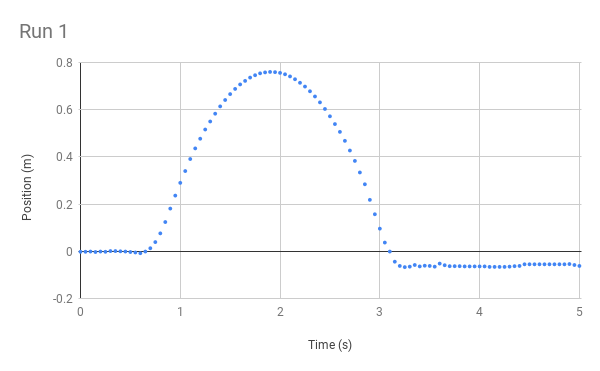
\includegraphics[scale=0.71]{image/02-incline/Run1-d.png}
    \caption{Full raw position data for run 1}
    \label{figure:02.raw.d}
\end{figure}
%%%%%%%%%%%%%%%%%%%%%%%%%%%%%%%%%%%%%%%%%%%%%%%%%%%%%%%%%%%%%%%%%%%%%%%%%%%%%%%%
\begin{figure}[ht]
    \centering
    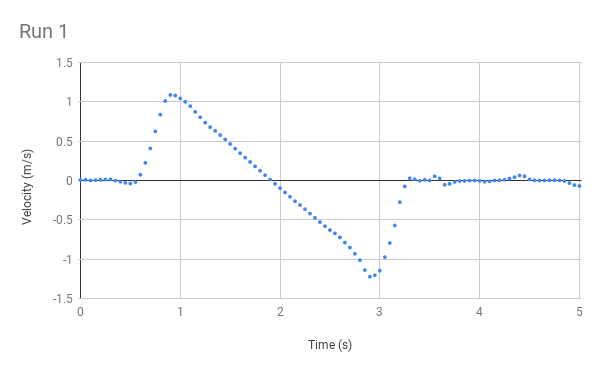
\includegraphics[scale=0.71]{image/02-incline/Run1-v.png}
    \caption{Full raw velocity data for run 1}
    \label{figure:02.raw.v}
\end{figure}
%%%%%%%%%%%%%%%%%%%%%%%%%%%%%%%%%%%%%%%%%%%%%%%%%%%%%%%%%%%%%%%%%%%%%%%%%%%%%%%%
\begin{figure}[ht]
    \centering
    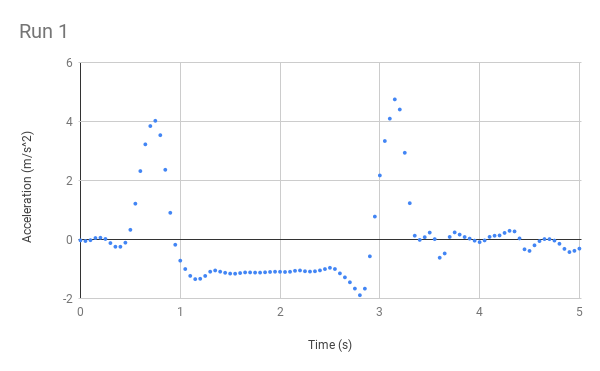
\includegraphics[scale=0.71]{image/02-incline/Run1-a.png}
    \caption{Full raw acceleration data for run 1}
    \label{figure:02.raw.a}
\end{figure}
%%%%%%%%%%%%%%%%%%%%%%%%%%%%%%%%%%%%%%%%%%%%%%%%%%%%%%%%%%%%%%%%%%%%%%%%%%%%%%%%
\begin{figure}[ht]
    \centering
    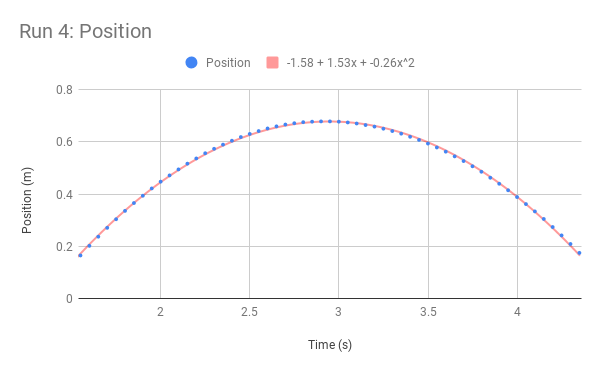
\includegraphics[scale=0.71]{image/02-incline/Run-4-d.png}
    \caption{Quadratic fit of position data for run 4}
    \label{figure:02.fit.d}
\end{figure}
%%%%%%%%%%%%%%%%%%%%%%%%%%%%%%%%%%%%%%%%%%%%%%%%%%%%%%%%%%%%%%%%%%%%%%%%%%%%%%%%
\begin{figure}[ht]
    \centering
    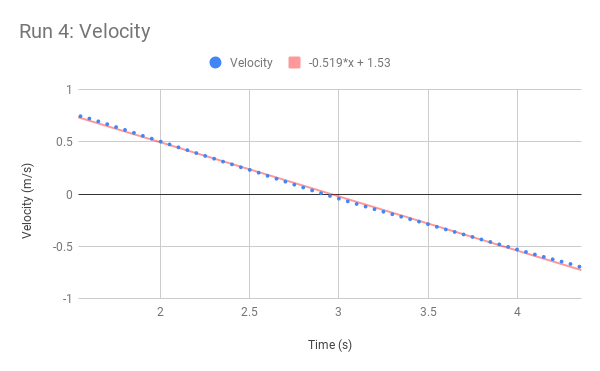
\includegraphics[scale=0.71]{image/02-incline/Run-4-v.png}
    \caption{Linear fit of velocity data for run 4}
    \label{figure:02.fit.v}
\end{figure}
%%%%%%%%%%%%%%%%%%%%%%%%%%%%%%%%%%%%%%%%%%%%%%%%%%%%%%%%%%%%%%%%%%%%%%%%%%%%%%%%